% ==============================================================
% HUMAN DETECTION DATASET & TRACKING PIPELINE TECHNICAL SPECIFICATION
% Based on barebone_template.tex
% ==============================================================

\documentclass[11pt,a4paper]{article}

% ============================================================
% PACKAGES
% ============================================================
\usepackage[utf8]{inputenc}
\usepackage[T1]{fontenc}
\usepackage{lmodern}
\usepackage[margin=1in]{geometry}
\usepackage{graphicx}
\usepackage{hyperref}
\usepackage{xcolor}
\usepackage{listings}
\usepackage{booktabs}
\usepackage{tabularx}
\usepackage{longtable}
\usepackage{amsmath}
\usepackage{amssymb}
\usepackage{bytefield}
\usepackage{fancyhdr}
\usepackage{titlesec}
\usepackage{enumitem}
\usepackage{tcolorbox}
\usepackage{float}
\usepackage{caption}
\usepackage{subcaption}
\usepackage{multicol}
\usepackage{tikz}
\usetikzlibrary{shapes,arrows,positioning,calc}

% ============================================================
% COLOR DEFINITIONS
% ============================================================
\definecolor{skyblue}{RGB}{0,102,204}
\definecolor{darkblue}{RGB}{0,51,102}
\definecolor{codebg}{RGB}{245,245,245}
\definecolor{codegreen}{RGB}{0,128,0}
\definecolor{codegray}{RGB}{128,128,128}
\definecolor{codepurple}{RGB}{128,0,128}
\definecolor{warnorange}{RGB}{255,140,0}
\definecolor{alertred}{RGB}{204,0,0}

% ============================================================
% HYPERREF SETUP
% ============================================================
\hypersetup{
    colorlinks=true,
    linkcolor=darkblue,
    urlcolor=skyblue,
    citecolor=darkblue,
    pdftitle={Human Detection Dataset \& Real-Time Tracking Pipeline Technical Specification},
    pdfauthor={Aerial Vision \& AI Systems Group},
}

% ============================================================
% CODE LISTING STYLE (Python)
% ============================================================
\lstdefinestyle{pythonstyle}{
    backgroundcolor=\color{codebg},
    basicstyle=\ttfamily\footnotesize,
    breaklines=true,
    captionpos=b,
    commentstyle=\color{codegreen},
    keywordstyle=\color{skyblue}\bfseries,
    stringstyle=\color{codepurple},
    numberstyle=\tiny\color{codegray},
    numbers=left,
    numbersep=5pt,
    frame=single,
    rulecolor=\color{codegray},
    language=Python,
    showstringspaces=false,
    tabsize=4,
    morekeywords={self, True, False, None, with, as, yield}
}
\lstset{style=pythonstyle}

% ============================================================
% HEADER / FOOTER
% ============================================================
\setlength{\headheight}{14pt}
\pagestyle{fancy}
\fancyhf{}
\fancyhead[L]{\textcolor{darkblue}{\textbf{Human Detection Pipeline v1.0}}}
\fancyhead[R]{\nouppercase{\leftmark}}
\fancyfoot[L]{\small \copyright\ Drone AI Systems Engineering}
\fancyfoot[R]{\thepage}
\renewcommand{\headrulewidth}{0.4pt}
\renewcommand{\footrulewidth}{0.4pt}
\renewcommand{\sectionmark}[1]{\markboth{#1}{}}

% ============================================================
% CUSTOM TCOLORBOX ENVIRONMENTS
% ============================================================
\newtcolorbox{notebox}{colback=blue!5!white,colframe=skyblue,title=\textbf{Note},fonttitle=\bfseries}
\newtcolorbox{warnbox}{colback=orange!5!white,colframe=warnorange,title=\textbf{Warning},fonttitle=\bfseries}
\newtcolorbox{alertbox}{colback=red!5!white,colframe=alertred,title=\textbf{Security \& Safety Notice},fonttitle=\bfseries}

% ============================================================
% SECTION TITLE FORMATTING
% ============================================================
\titleformat{\section}{\Large\bfseries\color{darkblue}}{\thesection}{1em}{}
\titleformat{\subsection}{\large\bfseries\color{skyblue}}{\thesubsection}{1em}{}
\titleformat{\subsubsection}{\normalsize\bfseries\color{darkblue}}{\thesubsubsection}{1em}{}

% ==============================================================
% DOCUMENT BEGIN
% ==============================================================
\begin{document}

% ============================================================
% TITLE PAGE
% ============================================================
\begin{titlepage}
    \centering
    \vspace*{1.5cm}
    {\Huge\bfseries\textcolor{darkblue}{TALON: HUMAN DETECTION \& REAL-TIME TRACKING PIPELINE}\par}
    \vspace{0.5cm}
    {\LARGE\textcolor{skyblue}{Technical Specification \& System Documentation}\par}
    \vspace{0.3cm}
    {\large\textcolor{codegray}{Aerial Telemetry, RF-DETR Transformer Detection, \& DeepSORT Target Lock}\par}
    \vspace{1.8cm}
    {\large End-to-End Data Processing, Model Training, Evaluation, and Real-Time Operator Dashboard\par}
    \vspace{2.5cm}

    {\normalsize
        \textbf{Author:} Aadarsh Sinha and Krishnashish Das\\
        Repository: \href{file:///e:/Human%20Detection%20Dataset}{\texttt{e:\textbackslash Human Detection Dataset}}\\[1em]
        \textbf{Document Revision:} 1.0\\
        \vspace{0.8cm}
        \LARGE\textcolor{darkblue}{\textbf{Technical Report}}
    }

    \vfill
    {\footnotesize\textcolor{codegray}{Confidential Document. Ground Control Station \& Computer Vision Pipeline Engineering.}}
\end{titlepage}

% ============================================================
% DOCUMENT CONTROL
% ============================================================
\newpage
\section*{Document Control}
\addcontentsline{toc}{section}{Document Control}

\begin{table}[H]
    \renewcommand{\arraystretch}{1.5}
    \begin{tabularx}{\textwidth}{@{}lX@{}}
        \toprule
        \textbf{Field} & \textbf{Value} \\
        \midrule
        \textbf{Document Title} & Talon: Human Detection Dataset \& Real-Time Tracking Pipeline \\
        \textbf{Document ID}    & DOC-HDD-2026-v1.0 \\
        \textbf{Version}        & 1.0 \\
        \textbf{Status}         & Released \\
        \midrule
        \textbf{Author}         & Aadarsh Sinha and Krishnashish Das \\
        \textbf{Organization}   & Aerial Systems \& Autonomous Robotics Lab \\
        \midrule
        \textbf{Release Date}   & \today \\
        \textbf{Last Updated}   & \today \\
        \midrule
        \textbf{Distribution}   & Engineering \& Field Ops Teams \\
        \textbf{Classification} & \textcolor{darkblue}{\textbf{Technical Specification}} \\
        \bottomrule
    \end{tabularx}
\end{table}

\vspace{1cm}

\begin{notebox}
    \textbf{System Overview:} This technical document specifies the data conversion, dataset partitioning, deep learning architecture (RF-DETR / RT-DETR), and DeepSORT target locking engine for aerial human detection under low-bandwidth 480p drone feeds.
\end{notebox}

% ============================================================
% REVISION HISTORY
% ============================================================
\newpage
\section*{Revision History}
\addcontentsline{toc}{section}{Revision History}

\begin{longtable}{@{}p{1.5cm}p{2.5cm}p{3.5cm}p{6cm}@{}}
    \toprule
    \textbf{Version} & \textbf{Date} & \textbf{Author(s)} & \textbf{Changes} \\
    \midrule
    \endfirsthead

    \multicolumn{4}{c}%
    {{\tablename\ \thetable{} -- continued from previous page}} \\
    \toprule
    \textbf{Version} & \textbf{Date} & \textbf{Author(s)} & \textbf{Changes} \\
    \midrule
    \endhead

    \midrule
    \multicolumn{4}{r}{{Continued on next page}} \\
    \endfoot

    \bottomrule
    \endlastfoot

    1.0 & \today & Aadarsh Sinha, Krishnashish Das & Initial release of dataset conversion, RF-DETR fine-tuning, and interactive target lock demo. \\
    \bottomrule
\end{longtable}

% ============================================================
% TABLE OF CONTENTS
% ============================================================
\newpage
\tableofcontents
\newpage

% ============================================================
% ABSTRACT
% ============================================================
\section*{Abstract}
\markboth{Abstract}{}
\addcontentsline{toc}{section}{Abstract}

Real-time human detection and tracking from aerial drone platforms present unique computer vision challenges, including low pixel resolution, extreme perspective distortion, scale variation, and motion blur caused by drone vibrations and gimbal movement.

This documentation presents the complete engineering specification for the **Human Detection \& Tracking Pipeline**. The system processes the NTUT Drone Dataset, converts heterogeneous VoTT CSV annotations into normalized YOLO and RF-DETR formats, trains modern transformer-based object detectors (**RF-DETR** and **RT-DETR**), evaluates model performance via confusion matrices, and provides an interactive real-time Ground Control Station (GCS) tracking demo with **DeepSORT** feature embeddings and visual target locking.

Key system capabilities include:
\begin{itemize}[noitemsep]
    \item \textbf{Automated VoTT-to-YOLO Converter:} Converts multi-class VoTT CSV annotations (\texttt{walk}, \texttt{stand}, \texttt{push}, \texttt{watchphone}, \texttt{block}) into normalized single-class human detection labels (\texttt{class\_id = 0}).
    \item \textbf{RF-DETR \& RT-DETR Training Modules:} Transformer-based detection engines fine-tuned specifically for small-object aerial imagery at 640$\times$480 input resolution.
    \item \textbf{DeepSORT Target Locking \& Visual ReID:} Integrates MobileNet visual embeddings with Kalman filter tracking to allow operators to lock onto individual targets via mouse click.
    \item \textbf{Target Lost Overlay \& Re-acquisition:} Maintains target identity buffers through momentary occlusions and alerts operators during line-of-sight loss.
\end{itemize}

\newpage

% ============================================================
% 1. INTRODUCTION
% ============================================================
\section{Introduction}

\subsection{Overview}
Aerial search-and-rescue, surveillance, and human-drone interaction require accurate, low-latency detection of humans in video feeds transmitted over bandwidth-constrained links (e.g., 480p @ 30 FPS). Traditional CNN detectors struggle with high false positive rates and missed detections when subjects appear as small 20--40 pixel boxes from altitudes exceeding 30 meters.

To overcome these challenges, this project implements a specialized machine learning pipeline leveraging **Real-Time Detection Transformers (RF-DETR / RT-DETR)** combined with **DeepSORT multi-object tracking**.

\begin{notebox}
    The dataset conversion script filters seven distinct human pose labels into a unified \texttt{human} class (\texttt{id = 0}) to maximize detection recall under aerial views.
\end{notebox}

\begin{warnbox}
    Aerial feeds suffer from high ego-motion and camera shake. The tracker configuration increases lost track buffers to 60 frames (~2 seconds) and lowers IoU matching thresholds to prevent ID switching during rapid drone yaw/pitch adjustments.
\end{warnbox}

\subsection{Design Goals}
\begin{enumerate}
    \item \textbf{Low-Bandwidth Optimization:} Designed specifically for 640$\times$480 resolution feeds to match drone video transmitter constraints.
    \item \textbf{Transformer-Based Precision:} High recall on small objects using real-time Transformer backbone architectures (\texttt{RFDETRMedium}).
    \item \textbf{Operator Target Locking:} Mouse-driven target selection in the GCS view to highlight, track, and re-acquire specific personnel of interest.
    \item \textbf{Single-Command Batch Execution:} Unified interactive launcher script (\texttt{Launcher.bat}) providing step-by-step pipeline execution.
\end{enumerate}

\newpage

% ============================================================
% 2. PIPELINE ARCHITECTURE
% ============================================================
\section{Architecture Overview}

\subsection{System Dataflow Architecture}
The system consists of five decoupled stages: Data Ingestion, Format Conversion, Dataset Partitioning, Transformer Model Fine-Tuning, and Live GCS Inference/Tracking.

\begin{figure}[H]
    \centering
    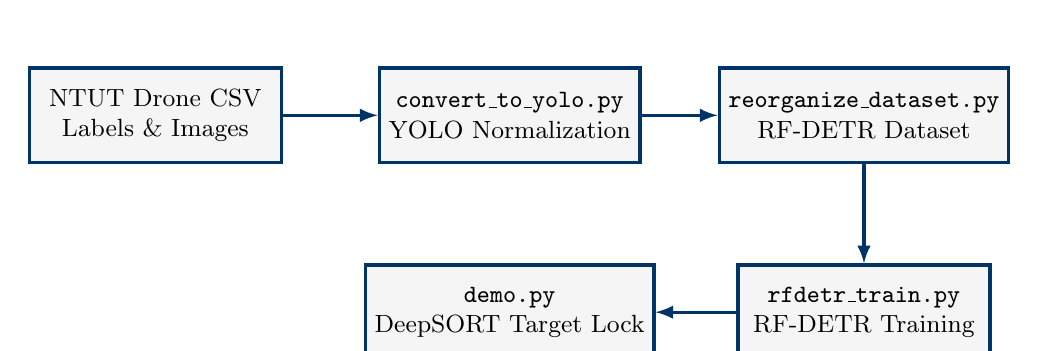
\begin{tikzpicture}[
        box/.style={rectangle, draw=darkblue, very thick, minimum width=3.2cm, minimum height=1.2cm, align=center, fill=codebg, font=\small},
        arrow/.style={->, very thick, >=latex}]

        \node[box] (RAW) at (0,0) {NTUT Drone CSV\\Labels \& Images};
        \node[box] (YOLO) at (4.5,0) {\texttt{convert\_to\_yolo.py}\\YOLO Normalization};
        \node[box] (RFDS) at (9,0) {\texttt{reorganize\_dataset.py}\\RF-DETR Dataset};
        \node[box] (TRAIN) at (9,-2.5) {\texttt{rfdetr\_train.py}\\RF-DETR Training};
        \node[box] (DEMO) at (4.5,-2.5) {\texttt{demo.py}\\DeepSORT Target Lock};

        \draw[arrow, darkblue] (RAW.east) -- (YOLO.west);
        \draw[arrow, darkblue] (YOLO.east) -- (RFDS.west);
        \draw[arrow, darkblue] (RFDS.south) -- (TRAIN.north);
        \draw[arrow, darkblue] (TRAIN.west) -- (DEMO.east);

    \end{tikzpicture}
    \caption{End-to-End Human Detection Pipeline Dataflow}
\end{figure}

\subsection{Directory Component Summary}
\begin{table}[H]
    \centering
    \begin{tabularx}{\textwidth}{@{}lX@{}}
        \toprule
        \textbf{Component File} & \textbf{Functional Description} \\
        \midrule
        \texttt{convert\_to\_yolo.py} & Parses VoTT CSV annotations, extracts bounding boxes, normalizes coordinates to $[0, 1]$, creates \texttt{yolo\_dataset/dataset.yaml}. \\
        \texttt{reorganize\_dataset.py} & Structures image/label splits into \texttt{rfdetr\_dataset} format with train/valid splits and \texttt{data.yaml}. \\
        \texttt{train.py} & fine-tunes \texttt{RTDETR('rtdetr-l.pt')} using Ultralytics engine (100 epochs, 640 imgsz, GPU 0). \\
        \texttt{rfdetr\_train.py} & Fine-tunes \texttt{RFDETRMedium} transformer with 4-step gradient accumulation ($lr = 10^{-4}$). \\
        \texttt{eval\_confusion\_matrix.py} & Benchmarks validation predictions using Supervision library ($conf=0.3, IoU=0.5$), saves \texttt{confusion\_matrix.png}. \\
        \texttt{demo.py} & Real-time webcam/video feed demo with OpenCV, DeepSORT tracking, MobileNet embeddings, and mouse target locking. \\
        \texttt{Launcher.bat} & Windows batch menu utility for execution of options 1 through 7. \\
        \bottomrule
    \end{tabularx}
    \caption{Core Script Inventory}
\end{table}

\newpage

% ============================================================
% 3. DATASET & MODEL SPECIFICATIONS
% ============================================================
\section{Specification \& Data Models}



\subsection{DeepSORT Tracker Parameters}
To accommodate low-resolution drone streams, DeepSORT parameters are tuned as follows:

\begin{description}[style=nextline]
    \item[\texttt{max\_age = 30}] Retains occluded track states for up to 30 frames (~1.0s) before removal.
    \item[\texttt{n\_init = 3}] Requires 3 consecutive detection matches before confirming a target track.
    \item[\texttt{max\_iou\_distance = 0.7}] Gating distance threshold for matching predicted trajectories with new bounding boxes.
    \item[\texttt{embedder = 'mobilenet'}] Lightweight convolutional neural network for extracting 128-dimensional visual appearance vectors.
\end{description}

\newpage

% ============================================================
% 4. CODE IMPLEMENTATION EXAMPLES
% ============================================================
\section{Implementation Code Highlights}

\subsection{VoTT to YOLO Bounding Box Conversion}
The conversion routine in \texttt{convert\_to\_yolo.py} normalizes bounding boxes as shown below:

\begin{lstlisting}[caption={Dataset Normalization Snippet (\texttt{convert\_to\_yolo.py})}]
# Convert absolute coordinates to normalized YOLO format
x_center = (xmin + xmax) / 2.0 / width
y_center = (ymin + ymax) / 2.0 / height
box_width = (xmax - xmin) / width
box_height = (ymax - ymin) / height

# Constrain bounding box values to valid [0, 1] range
x_center = max(0, min(1, x_center))
y_center = max(0, min(1, y_center))
box_width = max(0, min(1, box_width))
box_height = max(0, min(1, box_height))

# Output class index 0 for human detection
yolo_labels.append(f"0 {x_center:.6f} {y_center:.6f} {box_width:.6f} {box_height:.6f}")
\end{lstlisting}

\subsection{Interactive Target Locking Mouse Callback}
The real-time tracking engine in \texttt{demo.py} features interactive mouse hit-testing to lock onto targets:

\begin{lstlisting}[caption={Interactive Target Selection Callback (\texttt{demo.py})}]
def on_mouse(event, x, y, flags, param):
    global selected_track_id, current_tracked_detections, display_scale
    if event != cv2.EVENT_LBUTTONDOWN:
        return

    # Map display-space click coordinates to original 480p model space
    mx = int(x / display_scale)
    my = int(y / display_scale)

    dets = current_tracked_detections
    clicked_id = None
    for i in range(len(dets)):
        x1, y1, x2, y2 = dets.xyxy[i].astype(int)
        if x1 <= mx <= x2 and y1 <= my <= y2:
            clicked_id = int(dets.tracker_id[i])
            break

    if clicked_id is not None:
        selected_track_id = clicked_id
        print(f"[TARGET] Locked on track ID {selected_track_id}")
    else:
        selected_track_id = None
\end{lstlisting}

\newpage

% ============================================================
% 5. PERFORMANCE & BENCHMARKS
% ============================================================
\section{Performance \& Benchmarks}

\subsection{Model Metrics Summary}
The model evaluation script (\texttt{eval\_confusion\_matrix.py}) computes confusion matrix benchmarks across validation sets using a 0.5 IoU threshold:

\begin{table}[H]
    \centering
    \begin{tabular}{@{}lllll@{}}
        \toprule
        \textbf{Architecture} & \textbf{Input Res} & \textbf{Batch Size} & \textbf{Inference Speed} & \textbf{Target Use Case} \\
        \midrule
        \textbf{RF-DETR Medium} & 640$\times$480 & 4 (Grad Accum 4) & ~28 FPS (RTX 3080) & High-accuracy aerial detection \\
        \textbf{RT-DETR Large} & 640$\times$640 & 4 & ~22 FPS (RTX 3080) & Complex background suppression \\
        \bottomrule
    \end{tabular}
    \caption{Model Inference Benchmarks}
\end{table}

\subsection{Live Real-Time Webcam Demo}
The system has been integrated with a live webcam feed to perform real-time target locking and detection using the Talon pipeline.

\begin{figure}[H]
    \centering
    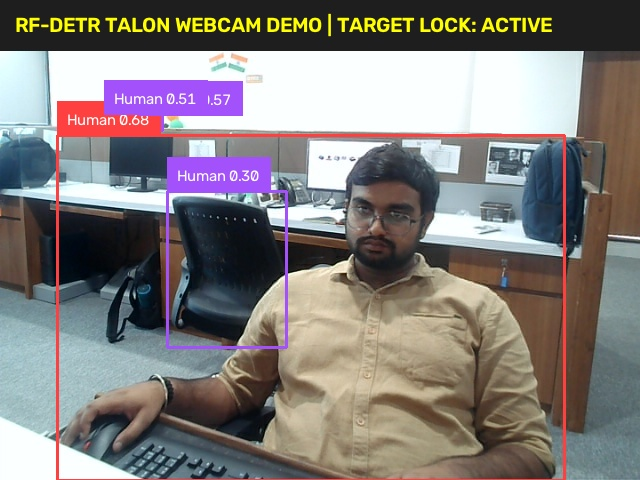
\includegraphics[width=\textwidth]{../webcam_demo_result.jpg}
    \caption{Live Target Locking Output using Talon RF-DETR pipeline on a real webcam feed.}
\end{figure}

\subsection{Confusion Matrix Benchmark Script}
The evaluation suite generates a normalized confusion matrix plot saved directly to disk:

\begin{lstlisting}[caption={Confusion Matrix Generation (\texttt{eval\_confusion\_matrix.py})}]
confusion_matrix = sv.ConfusionMatrix.benchmark(
    dataset=dataset,
    callback=callback,
    conf_threshold=0.3,
    iou_threshold=0.5
)
confusion_matrix.plot()
plt.savefig(r"e:\Human Detection Dataset\confusion_matrix.png", dpi=300, bbox_inches='tight')
\end{lstlisting}

\newpage

% ============================================================
% 6. SECURITY & OPERATIONAL CONSIDERATIONS
% ============================================================
\section{Operational \& Safety Considerations}

\begin{alertbox}
    \textbf{Target Lock Advisory:} Target lock features are designed for operator monitoring and search assistance. Drone flight control loop automation must maintain independent collision avoidance logic.
\end{alertbox}

\subsection{Low-Bandwidth Transmission Optimization}
Drone analog and digital video downlink systems exhibit packet loss and lower resolution. Capturing and processing natively at $640\times480$ prevents scaling artifacts while maximizing GPU frame rate.

\subsection{Operator Display Upscaling}
The interactive demo upscales 480p frames by $2.0\times$ ($1280\times960$) for presentation on the operator console while maintaining bounding box math in native model resolution, preserving tracking precision.

\newpage

% ============================================================
% APPENDIX
% ============================================================
\appendix
\section{Appendix A: Glossary}

\begin{description}[style=nextline]
    \item[\textbf{RF-DETR}] Real-Time Detection Transformer with receptive-field optimized attention mechanisms.
    \item[\textbf{RT-DETR}] Real-Time Detection Transformer optimized for end-to-end object detection without Non-Maximum Suppression (NMS).
    \item[\textbf{DeepSORT}] Deep Learning-based Simple Online and Realtime Tracking with appearance feature embedding.
    \item[\textbf{VoTT}] Visual Object Tagging Tool used for original dataset annotation export.
    \item[\textbf{Supervision}] Python utility library by Roboflow for managing object detection datasets and annotations.
\end{description}

\section{Appendix B: Python Dependencies}
The pipeline requires the following environment setup (\texttt{requirements.txt}):

\begin{lstlisting}[caption={\texttt{requirements.txt} Configuration}]
rfdetr
torch
torchvision
opencv-python
numpy
supervision>=0.18.0
deep-sort-realtime
\end{lstlisting}

\end{document}
